\label{chap:methodology}

In this chapter the different data silos at \nomeHsl{} which are used for this work are discussed in detail and so forth. First, it is necessary to understand how data is partitioned in a hospital. 

For historical reasons the data is \emph{departmentalized} at most hospitals. For large institutions there is always at least four well defined databases: the Electronic Health Record (EHR) or Electronic Medical Record (EMR), the Radiology Information System (RIS), the Hospital Information System (HIS) and the Laboratory Information System (LIS).

\section{EHR: Electronic Health Record}
\label{sec:ehr}

It is often separated into a clinical data part and a Enterprise Resource Planning (ERP) parts which are linked by different institution aspects. The final end goal of the EHR is usually reimbursement purposes. For that matter, in the US the Diagnosis-related Group (DRG) which is based on the EHR information is the basis for patient related reimbursement purposes even in a value-based care model.

\subsection{Medical Payment Model and the Health Record}
\label{sec:ehr_payment}
In the USA, since 2015 the existence of a EHR in every clinic, hospital or local patient care provider is mandatory and it's inexistence can result in progressive penalties for Medicare and Medicaid reimbursements, starting at 1\% as of this year and increasing throughout the years.

Also, in 1996 the Health Insurance and Portability and Accountability Act (HIPAA) was introduced\cite{annasHipaa2003}. This created an environment where several smaller EHR manufacturer companies thrived. Later on, with several merges and acquisitions it happens that a market consolidation happened and is still happening for the United States of America.

In Brazil, the Public Health System (SUS) provides reimbursement based on a Fee For Service (FFS) model instead of Medicare's value-based care model. Thus, there is small benefit for several institutions to drive patient's cost down in the overall sense of it though private insurance companies have been vigilant of these aspects and recently some have been descredited from some of the key payers in the national system. The D'or network descredition from Amil was one such case for several of it's hospitals in São Paulo and Rio de Janeiro states became affected after the insurance company audited several of it's hospitals accounts\cite{amilRedeDor2019}.

\subsection{Patient Information}

\label{sec:ehr_patient_information}
\begin{center}
\begin{figure}
\begin{centering}
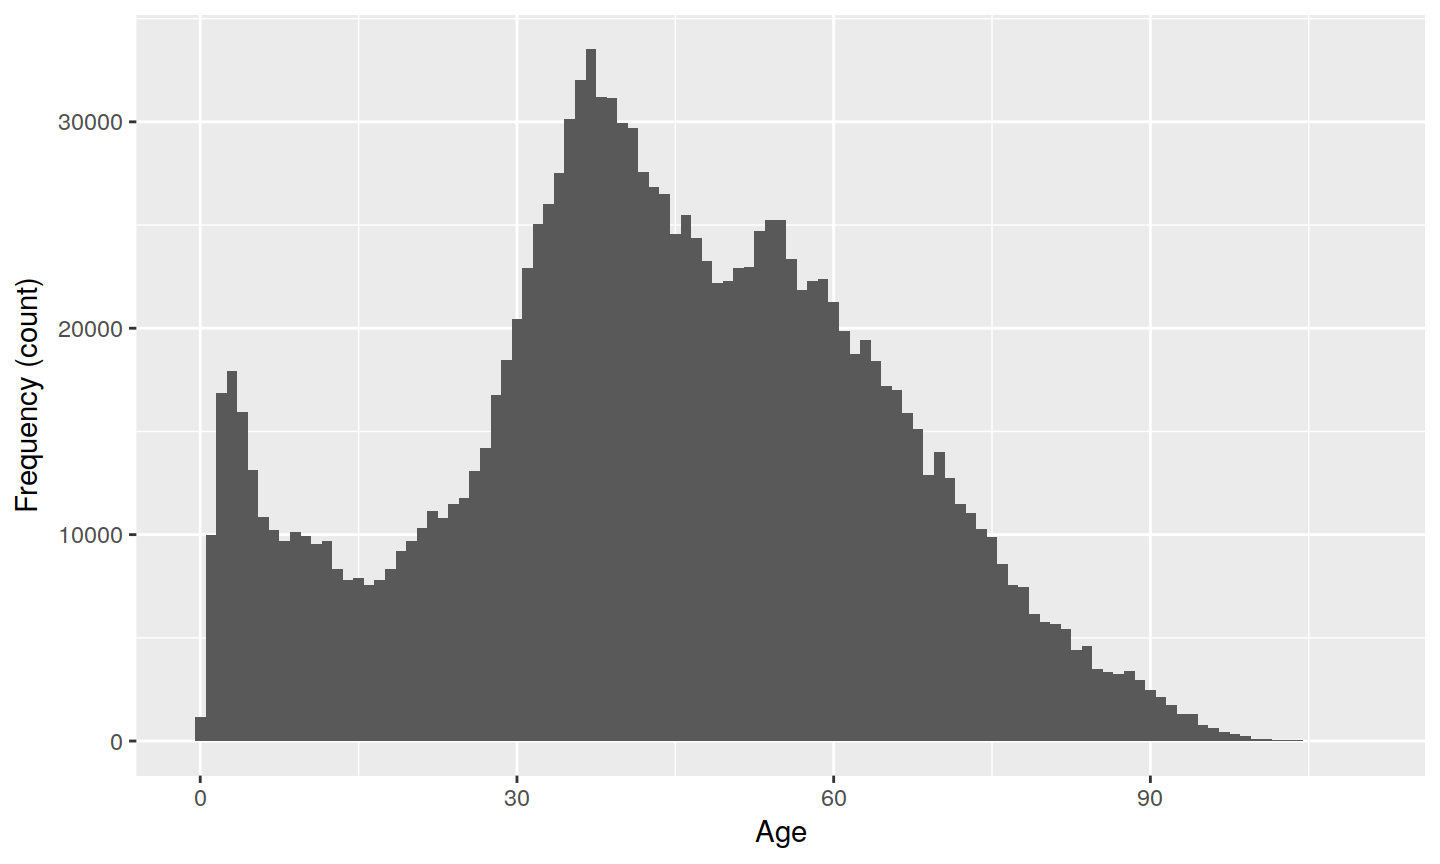
\includegraphics[width=0.5\textwidth]{PatientPopulation}
\par\end{centering}
\begin{centering}
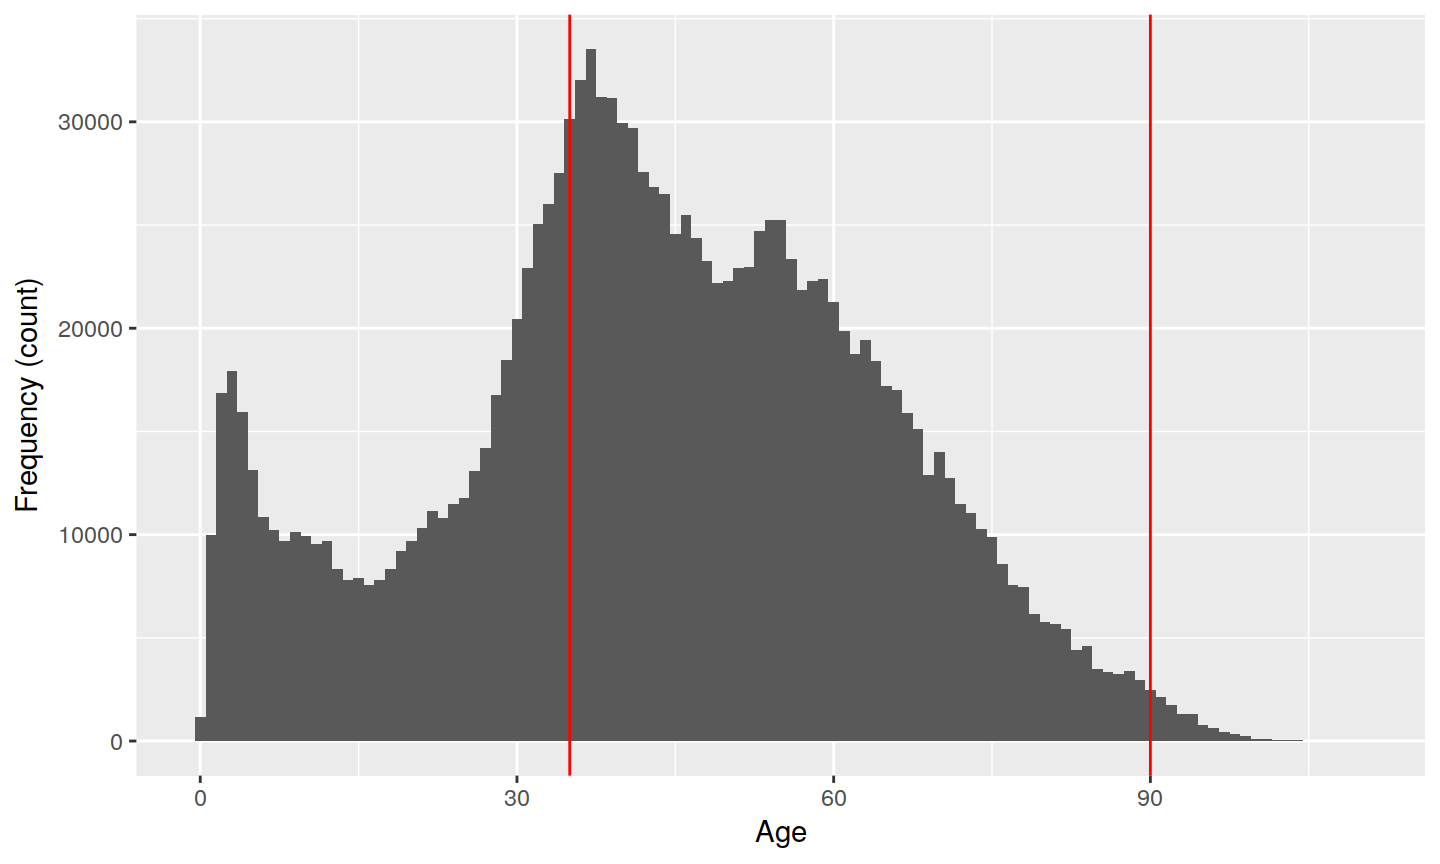
\includegraphics[width=0.49\textwidth]{PatientPopulationWithThreshold}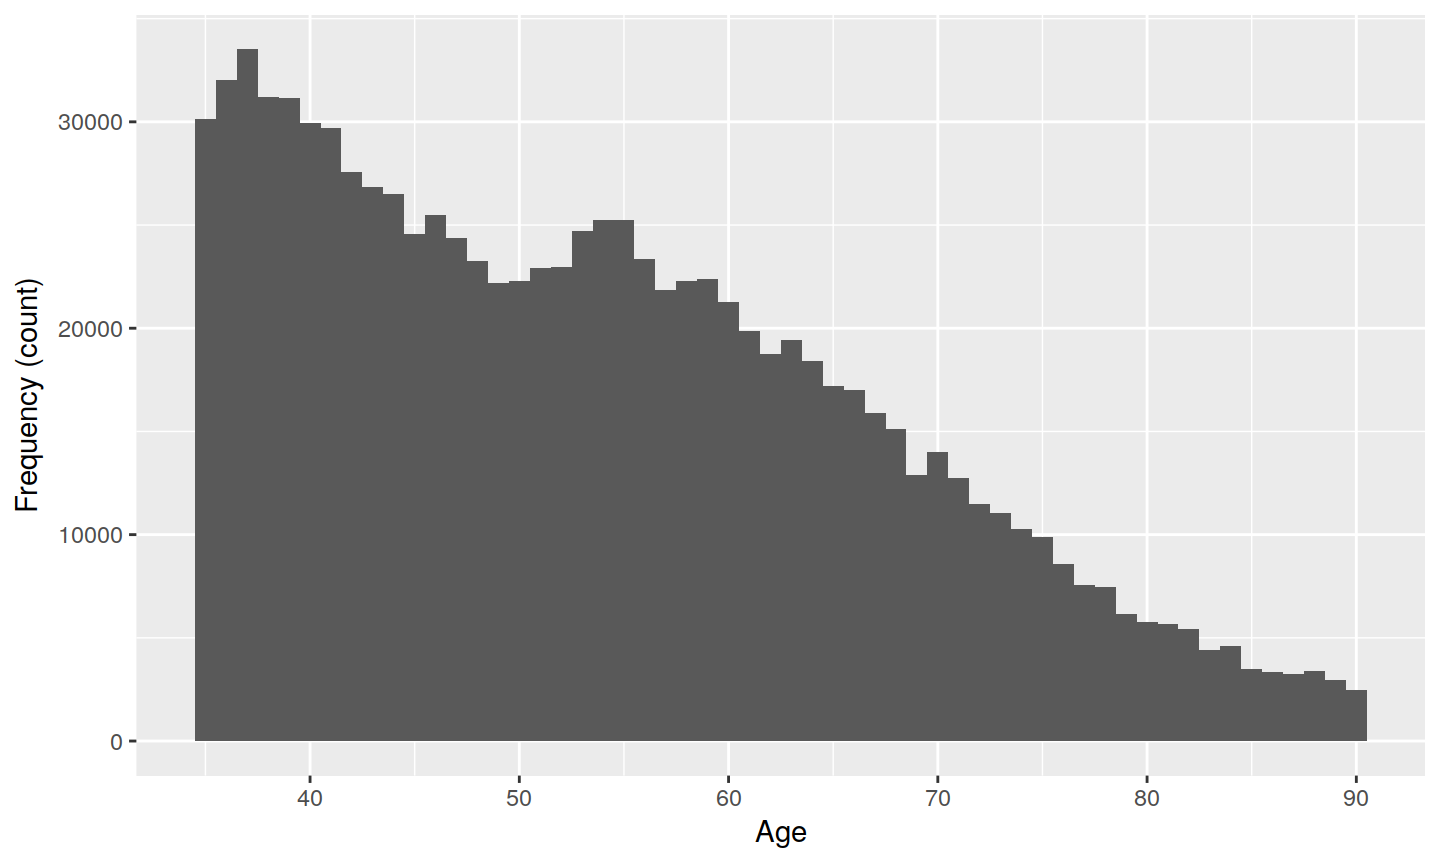
\includegraphics[width=0.49\textwidth]{FilteredLungNodulePopulation}
\end{centering}
\caption{\label{fig:patient_population}The upper histogram defines the whole \nomeHsl{} population. The lower left image shows a vertical bar on 35 and 90 years which can
be considered minimum and maximum bounds for patient screening and
finally the lower right image is a filtered version of the lower left
histogram only taking the age intereval of interest into consideration.}
\end{figure}
\vspace*{-38pt}
\end{center}

Due to the fact that the EHR is often also a ERP system it oftens contain both hospital storage, patient demographics, physician information, drug administration information and so on. 

At \nomeHsl{}, the EHR is Philips TASY which is one of the key players in the brazilian medical market. They also have an in-house developed EHR system called the Patient Electronic Portal (PEP) that is currently heavily used for the oncology department. All PEP information is exchanged and currently also stored as part of the TASY database.

The figure~\ref{fig:patient_population} displays the whole patient population for the institution which is constituted of all male and female patients in that institution. The whole population is more than a million patients from Brazil. Patients from other nationalities where ruled out. The patient identification inside of \nomeHslShort{} is a unique patient index which is common for all systems inside of this institution. In such cases, this is often called the Master Patient Index (MPI) and it is the enabler of all data queries, analytics and inferences that are part of this work.

\begin{center}
\begin{figure}
\begin{centering}
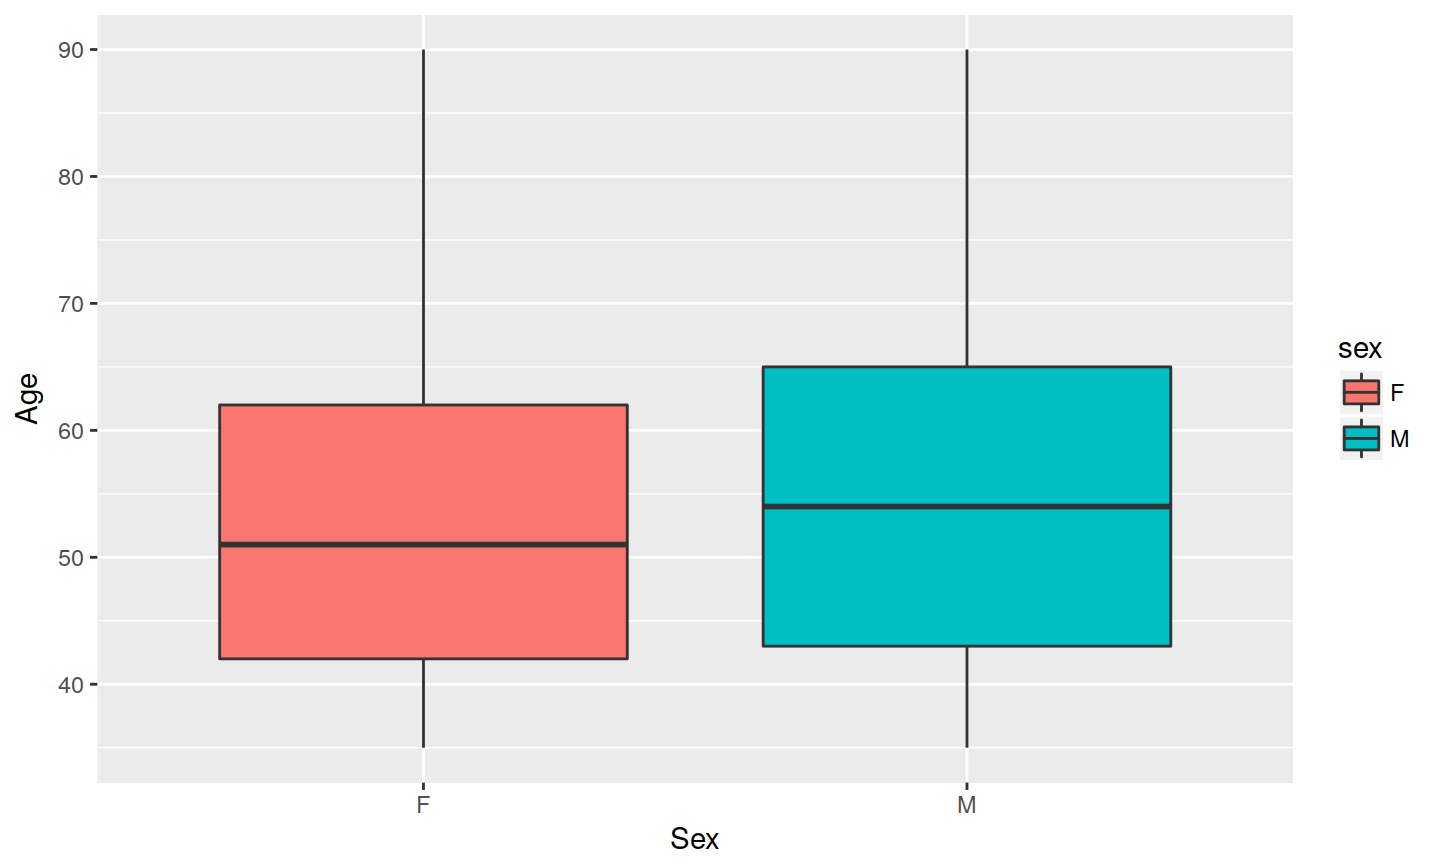
\includegraphics[width=1.0\textwidth]{PatientSexBoxplot}
\end{centering}
\caption{\label{fig:patient_sex_boxplot}The patient sexs boxplot for the age interval between 35 and 90 years.}
\end{figure}
\vspace*{-44pt}
\end{center}

\section{RIS: Radiology Information System}

In a typical institution all the radiology ordering and reporting is stored into the RIS, however for the images themselves, as a single exam can contain several thousand of DICOM monochromatic or colored images, a separate archiving for these are required. 

The Radiology is one of the most advanced departments where IT integration is related due to the sheer volume of raw information generated by this department in a daily basis. Also, screening and imaging exams are one of the most expensive and rentable parts of a hospital, especially in a FFS reimbursement model (see section~\ref{sec:ehr_payment} for further explanations).

\begin{center}
\begin{figure}
\begin{centering}
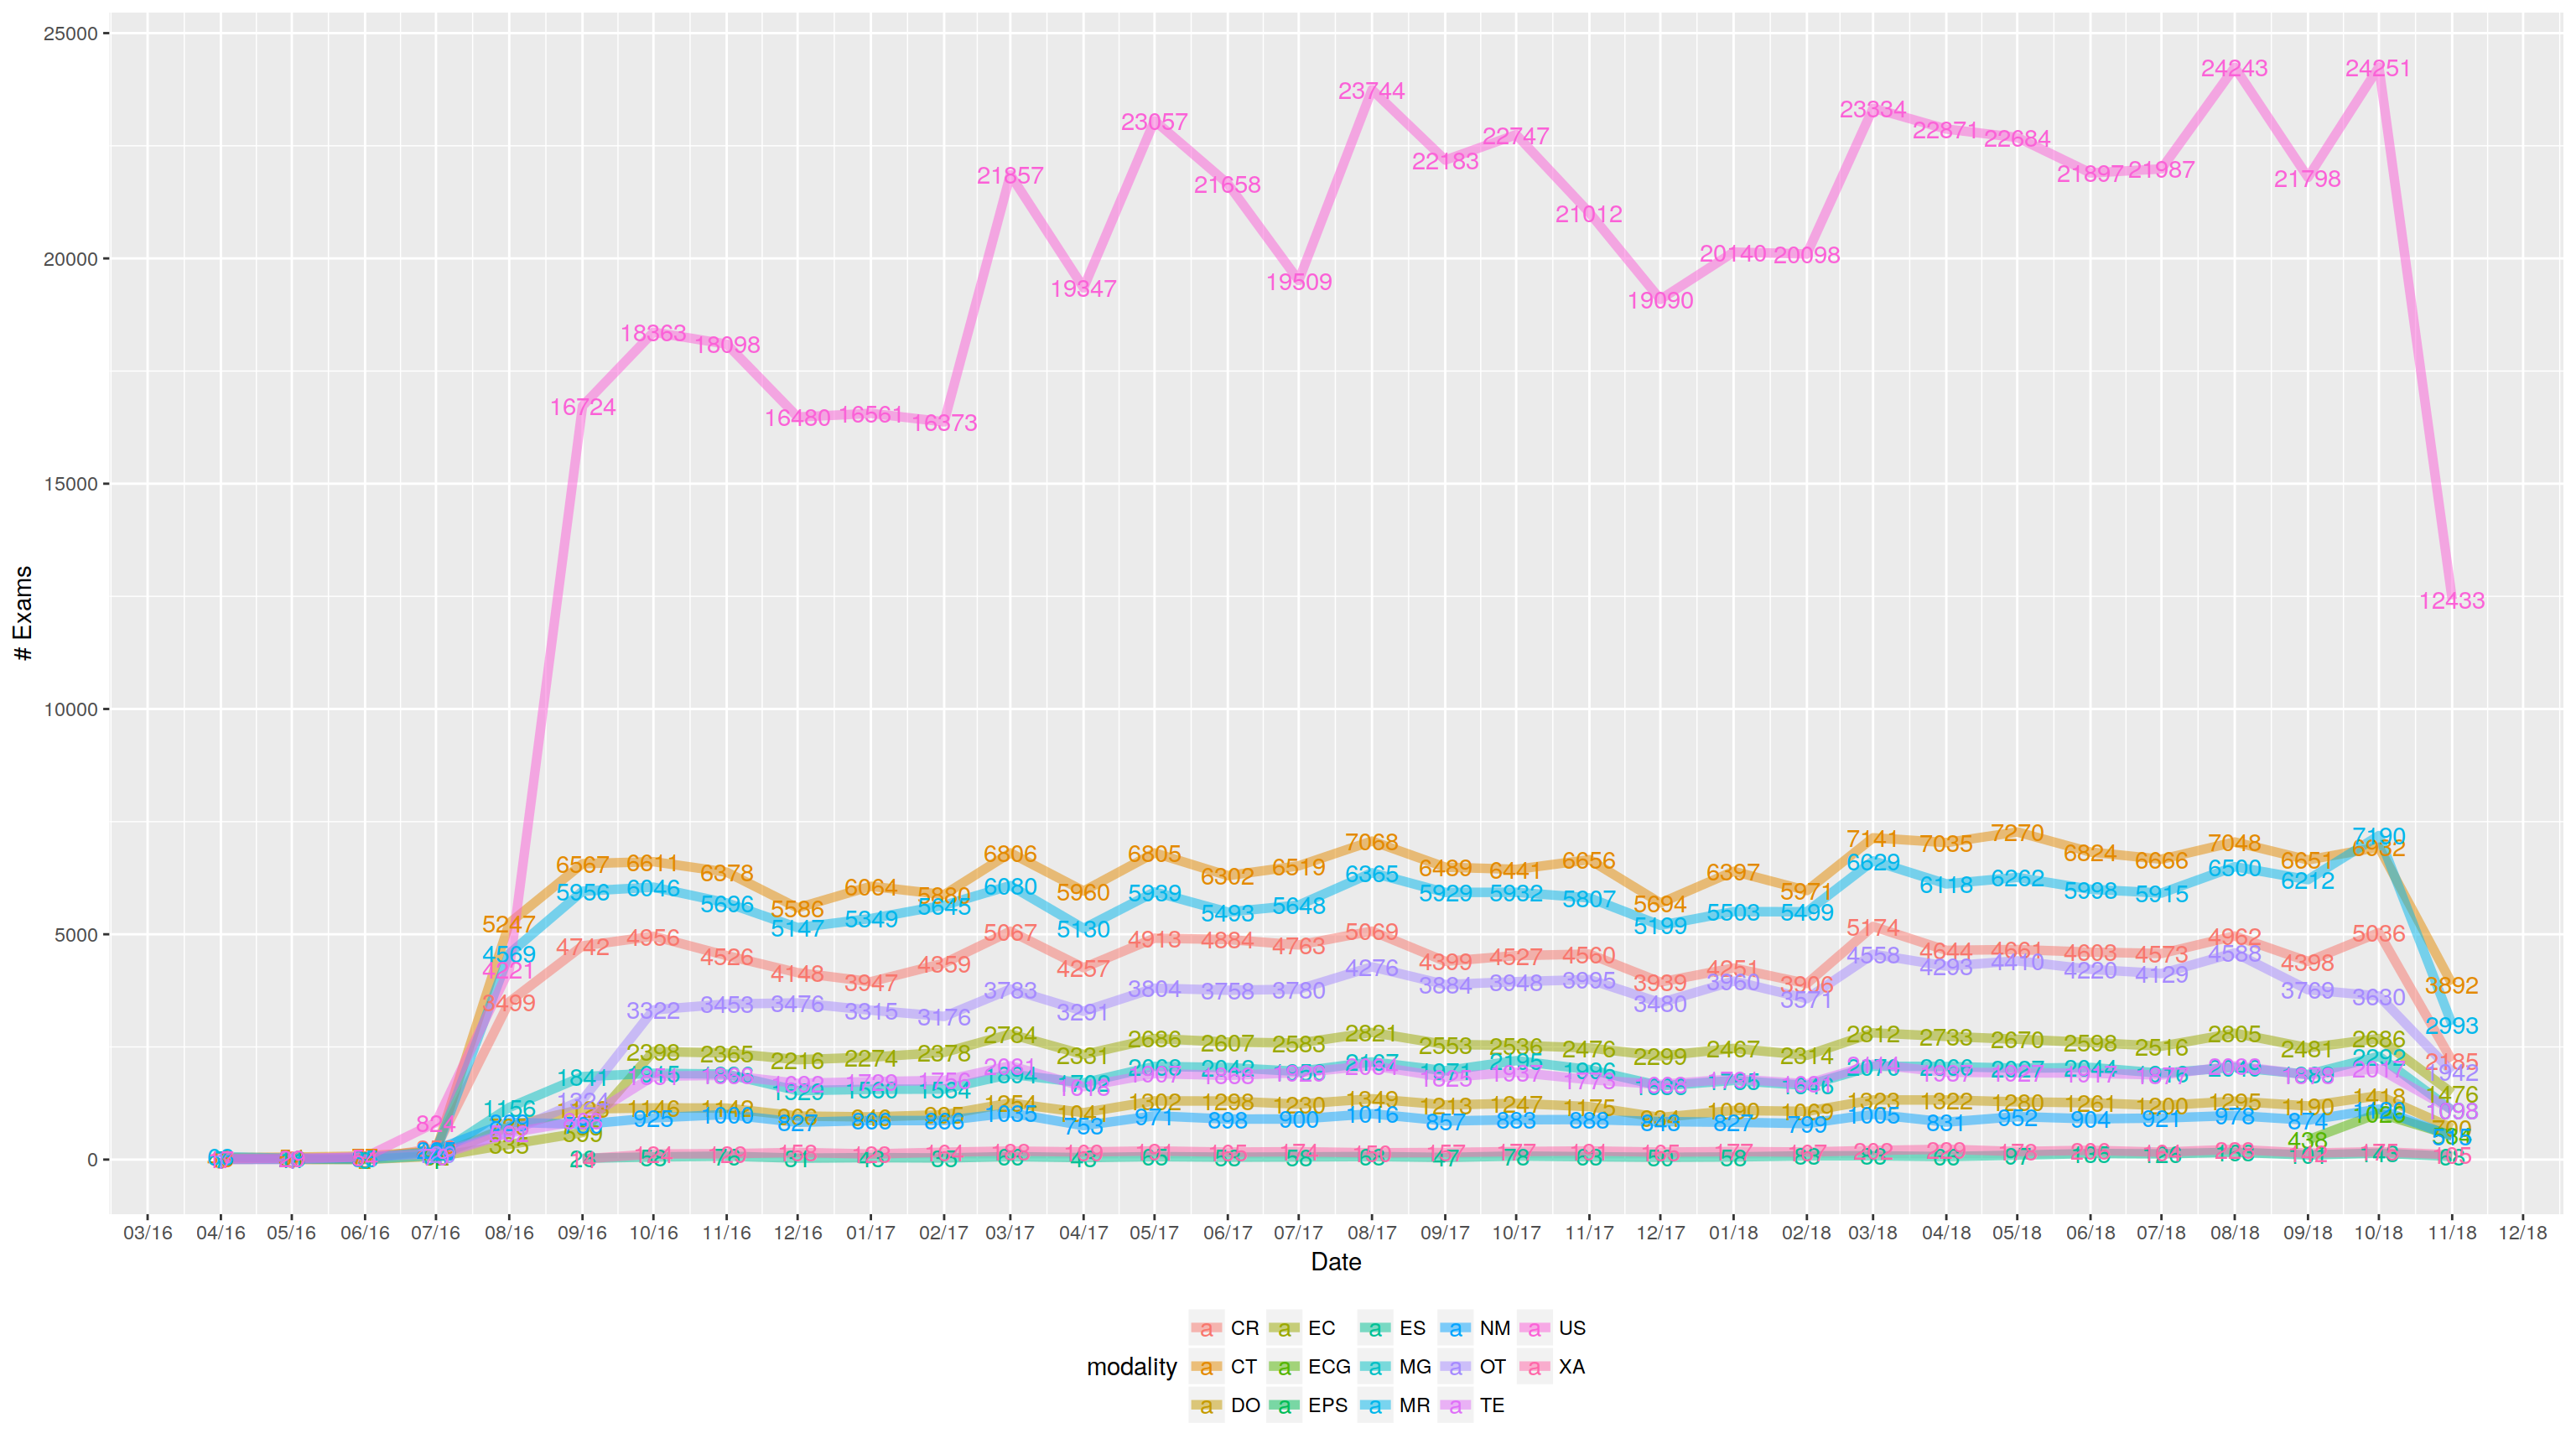
\includegraphics[width=1.0\textwidth]{RisExamsPerMonth}
\end{centering}
\caption{\label{fig:ris_exams_per_month} The number of exams per month that flows through the RIS in \nomeHslShort{} from January/2016 to December/2018.}
\end{figure}
\vspace*{-44pt}
\end{center}

This separate archive is the Picture Archiving and Communication System (PACS) which is part of the DICOM network protocol and is able to store DICOM images\cite{clunie2000, mildenberger2002}. In figure~\ref{fig:ris_exams_per_month}, one can see the sheer number of exams per month. Each of these can be constituted of up to several thousand images, so archiving is usually done in two-steps for these images: A short-term storage (STS) and a long-term archiving (LTA). The STS are usually only able to hold a few weeks of imaging data for the whole institution. The LTA in the other hand, can hold all the institutions information for as long as required by the country's regulatory.

The images themselves are target of various modern algorithms that try to extract meaningful clinical information from the images themselves. One simple way to do so is to use a suite of pretrained algorithms on an annotated image database, for example ImageNet\cite{deng2009}.

Although this sort of approach is very popular in the literature it does little to ensure that patients that never did an imaging at an institution will have an adequate follow up according to the suspected diagnosis and their clinical holistic scenario. For that matter, the integration to the EHR (section~\ref{sec:ehr}) is mandatory.

\section{HIS\@: Hospital Information System}

The HIS is a software system that is focused on the administrative parts of a medical institution, such as medical staff, financial, legal, documents and the processing of all services. 

Very often into hospitals and clinics the HIS tags along a local EHR installation and is very often a part of the same software package. This happens to be the case at \nomeHsl{}.

\section{LIS\@: Laboratory Information System}

The data silo that contains the most structured and ready-to-use information is the LIS\@. This contains all lab tests (such as blood tests, pathology tests, etc) performed to a patient and can also contain information related to the biling, the tracking of patient records, the analytical reporting of these tests and even sometimes an International Classification of Diseases (ICD) encoding for comparison of lab results.

The imaging and the lab departments are the ones that contain the most structured information out of all the departments in a medical institution. This makes these the easiest and most straightforward data silos to work with and extract information without requiring the usage of NLP techniques.

\section{Other Data Silos}

It is very often necessary to have complementary databases to fill in gaps in the different information systems available in an institution. Data replication is often very common for the medical institutions and it's consolidation has been known to be very hard and sometimes even department or condition specific, often requiring manual work steps to be done.

One of the key ways to extract patient meaningful historical information is through the different forms that a patient fills in an institution when visiting for a consultation or exams. These will often have semi-structured formats and their open fields can also frequently contain valuable clinical information. 

One of the key problems in that sense, is that very often the physician, nursing and technician notes on patients will contain useful information but are in a unstructured format. This is so due to historical reasons, even though the EHR systems have evolved quite a bit in the direction of having a more formal and structured information, very often clinical information is still written in a free text format, the same as it used to be in a pre-digital era where EHR systems where non existent and all the medical information was written in paper notes that had to be written, read and stored by clinical personnel.

Nowadays, it is very common that specific forms and patient outcome information is also present in the EHR, described in section~\ref{sec:ehr}. However, additional data silos are often present, including data marts, lakes and warehouses to store, mine and provide analytical clinical diagnosis and information on a regular basis.

\section{Integrating Data Silos: Patient Nodules and Smoking History}

The figure~\ref{fig:patient_population} shows the overall patient population for the institution. The suggested patient population filters are based on \nomeHslShort{} own internal guidelines along with the Fleischner 2017 and NCCN recommendations.

This is only possible by the fact that for every in-patient that performs a chest CT, a self reported patient addiction is obtained. From the \emph{patient habits and addictions} table, a list of tabagism self reported information is processed and the output is visualized in figure~\ref{fig:cigars_per_day}.
% TODO - most common answers tables
Also, a 10 pack-year smoking history qualifies the patient for a routine follow up after 35 years as mentioned for \nomeHslShort{}. An overall picture of the patient smoking behavior for the hospital's own population is given. In this dataset, only 24\% of all screeneable patients can be considered smokers which is only slightly lower than the wolrdwide average of 30\% smokers.

\begin{center}
\begin{figure}
\begin{centering}
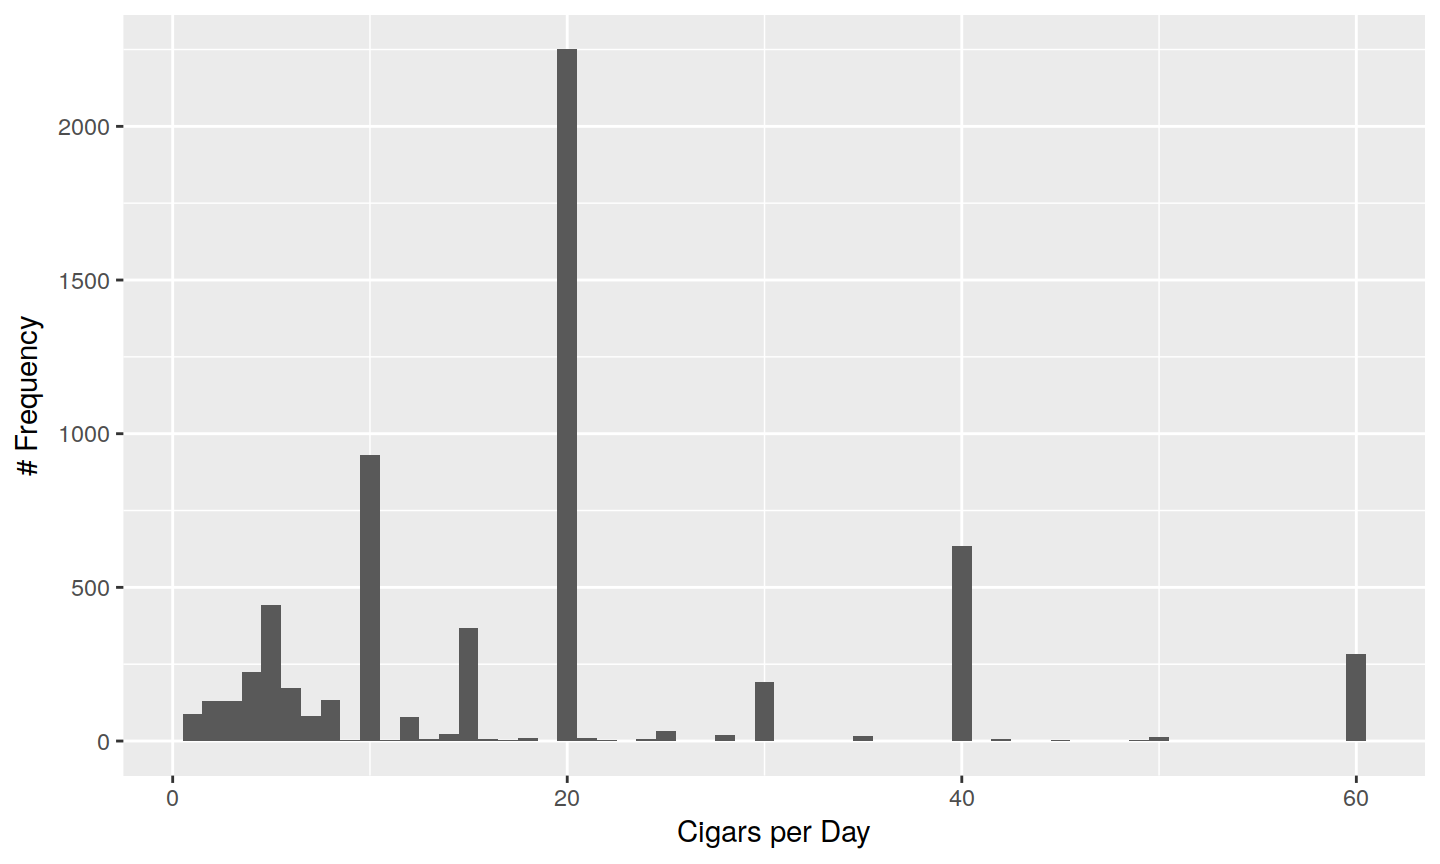
\includegraphics[width=1\textwidth]{PatientsCigarsPerDay}
\par\end{centering}
\caption{\label{fig:cigars_per_day} Histogram of cigars per day according to \nomeHsl{} patient self reported information.}
\end{figure}
\vspace*{-44pt}
\end{center}

This idea of following which patients have self reported tabagism information is useful for screening but the radiologists tend to report the incidental lung nodules in adherence with the Fleischner 2017 guideline. This means that it is also possible to extract from the radiology reports the information required to fill the Fleischner required parameters of nodule size, multiplicity, location and type as seen in tables~\ref{tab:solid_nodules} and~\ref{tab:subsolid_nodules}. 

The tabagism information from figure~\ref{fig:cigars_per_day} is a useful information to help stratify the patient risk profile. That means that there are two different \emph{risk profile} stratification guides: the nodule-centric risk and the patient-centric risk. Both contribute to the overall lung cancer malignancy risk stratification and can be considered part of Fleischner\cite{fleischner2017}. It is important to separate them as the patient risk profile is often obtained from self reported data, usually available in the EHR and the nodules evolution information is extracted directly from the radiology reports (RIS).

\subsection{Patient Risk Profile}

\begin{table}
\begin{centering}
\begin{tabular}{c|c|c|c}
\hline 
Risk & Age (years) & Smoking History & Screening \tabularnewline
\hline 
Very High & 55 to 74 & $\ge30$ pack years; quit $\le$15 years & Yes \tabularnewline
High & $\ge$50 & $\ge20$ pack years & Yes\tabularnewline 
Moderate & $\ge$50 & $\ge20$ pack years (second-hand smoke) & No \tabularnewline 
Low & $<$50 & $<20$ pack years & No\tabularnewline
\hline 
\end{tabular}
\end{centering}
\caption{\label{tab:nccn_risk_lung_nodule}A table that stratifies patients according to the NCCN lung screening
guidelines.}
\end{table}

\begin{center}
\begin{figure}
\begin{centering}
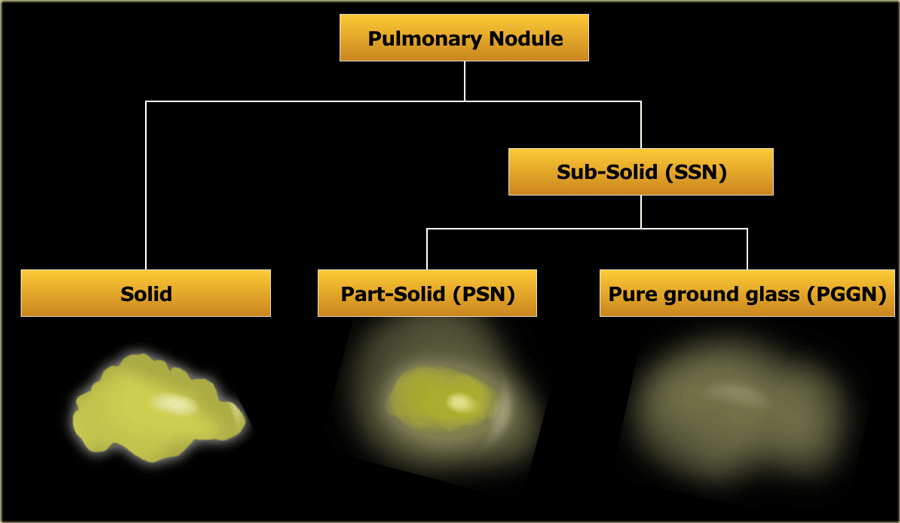
\includegraphics[width=1\textwidth]{Fleischner_PulmonaryNoduleTypes}
\par\end{centering}
\caption{\label{figh:fleischner_pulmonary_nodules_types}Nodule solid and sub-solid (SSN) types according to \citeonline{fleischner2017}.}
\end{figure}
\vspace*{-38pt}
\end{center}

There is a good overall agreement between different guidelines as shown in chapter~\ref{chap:literature_review} that the smoking history of a patient is one of the key aspects for lung cancer incidency and evolution. This is true for both NCCN and Fleischner guidelines. The table~\ref{tab:nccn_risk_lung_nodule} shows the risk profiles for each patient given their tabagism history. 

From Fleischner's perspective the key main patient centric factors that can contribute to lung cancer are:

\begin{itemize}
  \item History of heavy smoking
  \item Exposure to asbestos, radium or uranium
  \item Family history of lung cancer, prior cancer
  \item Older age
  \item Gender (Females > Male)
  \item Race (Black and native Hawaiian > White)
\end{itemize}

\subsection{Nodule Risk Profile}

The risk stratification directly from a nodule description is possible by applying directly the definitions from the Fleischner 2017 guideline. As described in the tables~\ref{tab:solid_nodules} and~\ref{tab:subsolid_nodules}, the parameters of interest are the nodule type, size, location and multiplicity. 

The nodule size and types are related as shown in figures~\ref{figh:fleischner_pulmonary_nodules_types} and~\ref{figh:fleischner_pulmonary_nodules_examples}. The first, shows the possible nodule types according to the overall solidity classification and the second shows what type of \emph{halos} are possible to find, especially in the sub-solid nodules (SSN).

\begin{center}
\begin{figure}
\begin{centering}
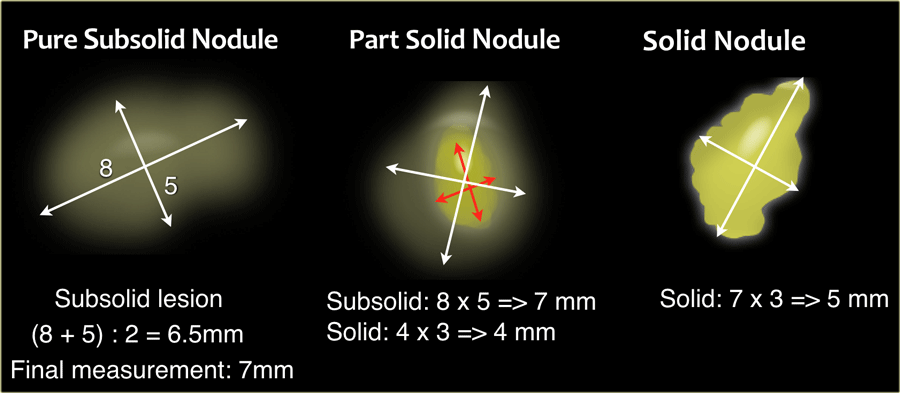
\includegraphics[width=1\textwidth]{Fleischner_PulmonaryNodulesExamples}
\par\end{centering}
\caption{\label{figh:fleischner_pulmonary_nodules_examples}Examples of pulmonary lung nodule classifications for pure sub-solid, part solid and solid nodules.}
\end{figure}
\vspace*{-38pt}
\end{center}

From Fleischner's perspective the key main nodules centric factors that can contribute to lung cancer are:

\begin{itemize}
  \item Marginal speculation 
  \item Upper lobe location
  \item Multiplicity ($<5$ nodules are less likely to have a malignancy risk)
  \item Rapid growth and increase in multiplicity
  \item Emphysema and pulmonary fibrosis (IPF)
\end{itemize}

It is often possible to extract these informations directly from a radiology report where the lungs are part of it. The most common type of reports where the lungs are also redacted as part of the image analysis are the chest tomography, abdomen tomography and the full body magnetic resonance imaging (MRI). Since the full-body MRIs constitute as little as 0.1\% of all imaging done at \nomeHslShort{}, then it is indeed of interest to exclude it from the overall analysis. This could be reviewed in the future as MRI are gaining traction as a non-invasive means of imaging due to the fact that it does not uses X-ray emission and thus does not imply into additional radiation exposure to the patient.

\begin{center}
\begin{figure}
\begin{centering}
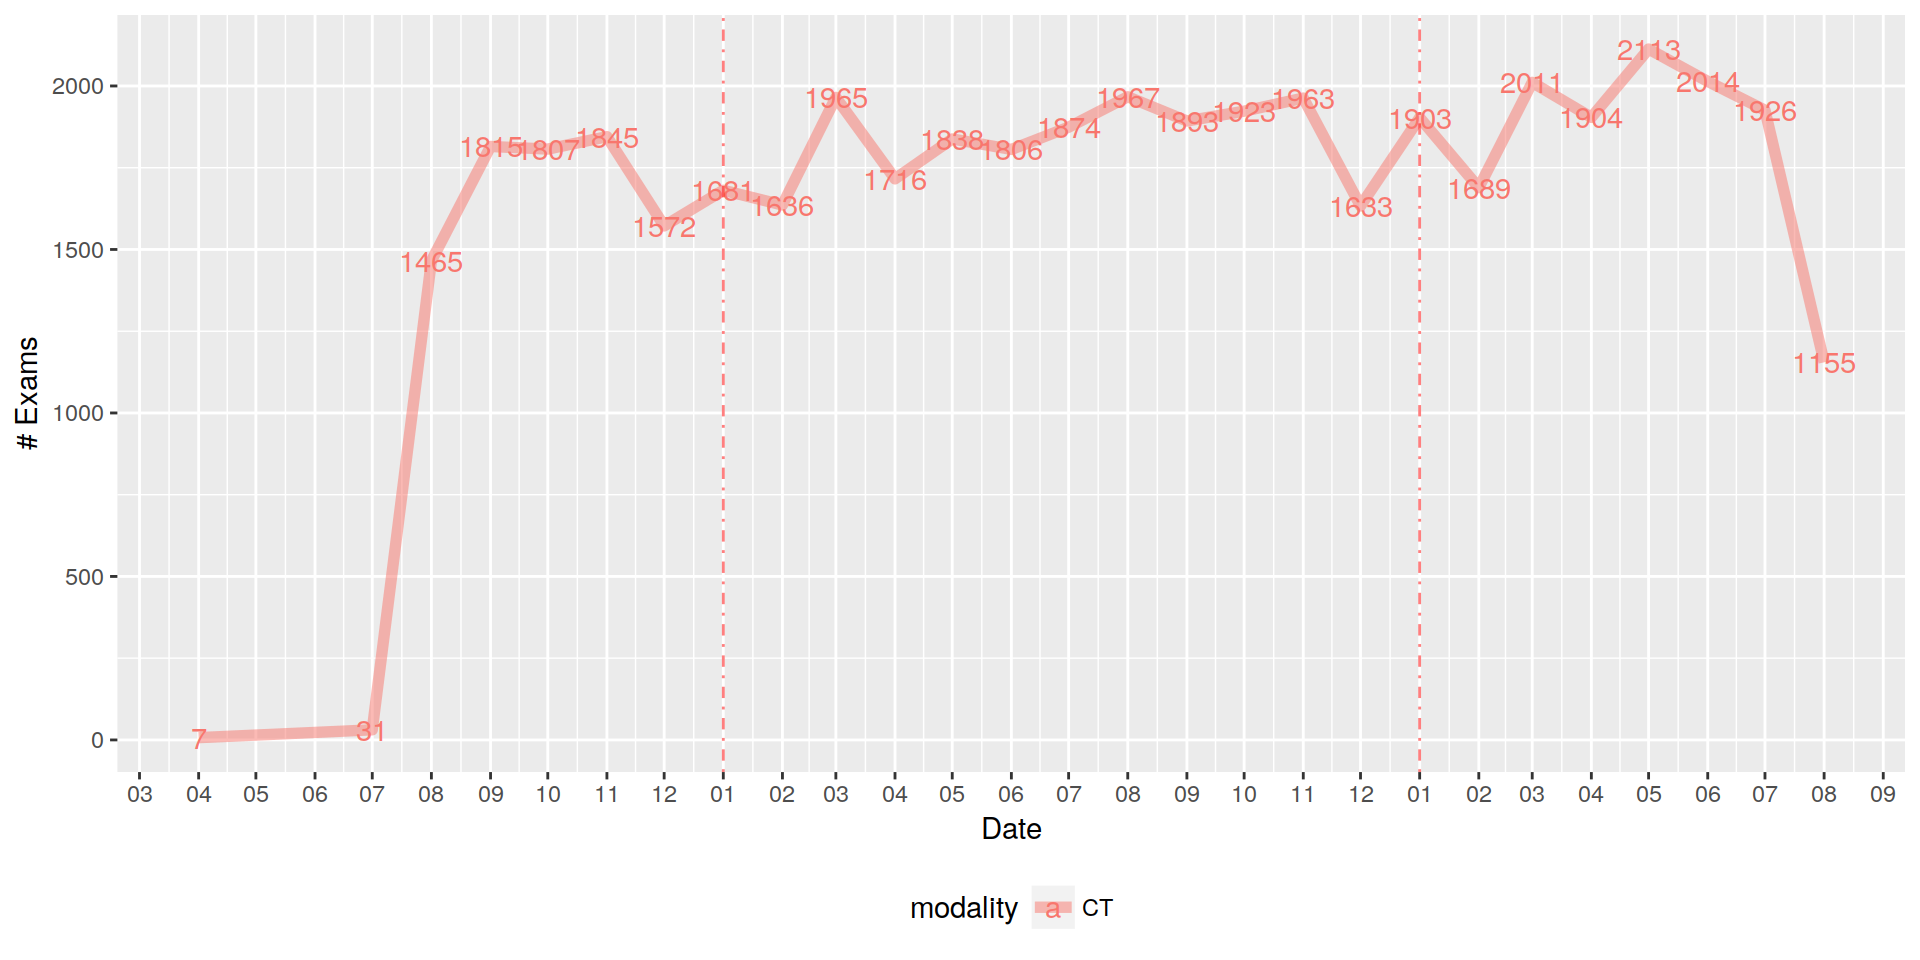
\includegraphics[width=1\textwidth]{RisCctExamsPerMonth}
\end{centering}
\caption{\label{fig:ris_cct_per_month}A display of the number of CCTs in the RIS system per month from January/2016 to September/2018. The vertical lines are year markers. It is noticeable the initial almost zero frequency at first which is because of the RIS implementation at the time (only regularized by 08/2016).}
\end{figure}
\vspace*{-38pt}
\end{center}
\section{Chest CT Reports} 

As seen in chapter~\ref{chap:literature_review}, the usage of LDCCT instead of traditional CCT can greatly increase the initial screening for incidental lung nodules and thus improve the early diagnosis of pulmonary cancer. However, due to reimbursement complexity and low availability in most institutions in Brazil it is very usual to have the use CCT to perform lung cancer screening.

This also holds true for \nomeHsl{}, so almost all of the radiology reports that were processed will fall on this case, save the patients where the ordering physician explicitly ordered the correct LDCCT exam to be performed. This is unfortunately the exception in the current \emph{status quo}.

CCT can also find a multitude of different nodules, so it is useful for liver, kidney, pancreas and vertebrae imaging. It is also one of the most common exams in any institution as it is greatly related to basic healthcare provisioning and Emergency Department screening as trauma patients will often get CCT or CXR exams as their first analysis.

\subsection{Analyzed Period}

All the following data analysis was conducted on the EHR and RIS systems by using the January/2016 to December/2018 information for both systems. However, the EHR information consists only of January/2016 up to August/2018 and the RIS information is only reliable from August/2016 to December/2018. In that sense, the intersection betweeen the two data silos timelines were used to avoid analysis problems. That means that the analyzed period consists of August/2016 to August/2018, or exactly two years of information. 

\subsection{CCT Report Processing}

To identify a patient population from the obtained radiology reports, it makes sense to use NLP to extract the nodule type, multiplicity and size from the reported sentences. The figure~\ref{fig:ris_cct_per_month} shows the number of CCTs processed in that institution per month. All these radiology reports sum up to 42,422 CCT reports. The next step is to understand how to process these reports.

From these approximately forty two thousand reports, only the ones with positive incidental lung nodule findings were extracted, resulting in \emph{29,586} reports in total. The total number of annotated sentences with incidental lung nodule findings were 36,127. 

\begin{center}
\begin{figure}
\begin{centering}
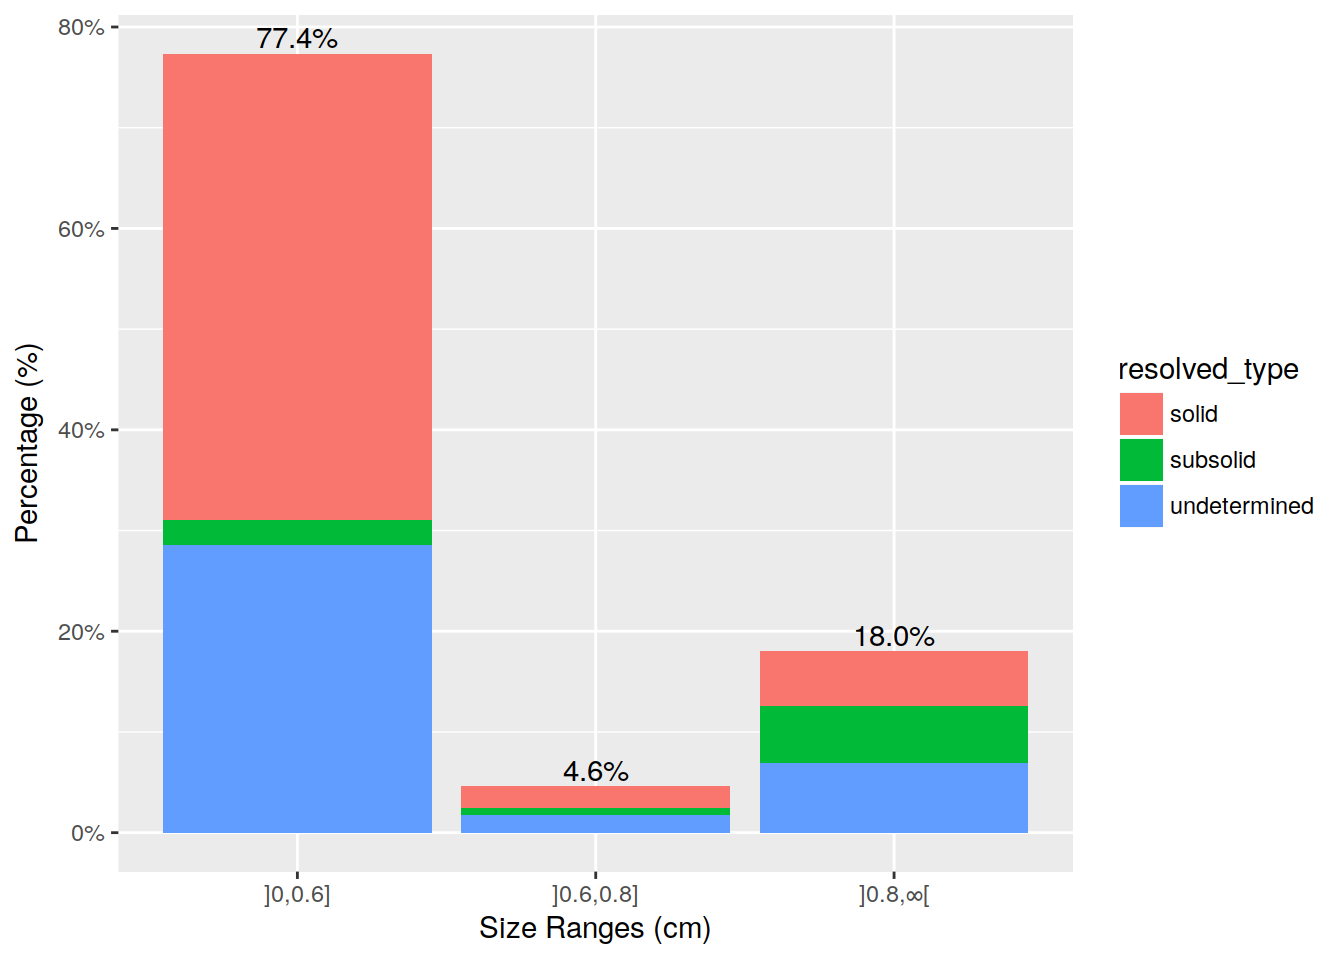
\includegraphics[height=0.26\textheight]{Reports_LungNoduleTypeSize}
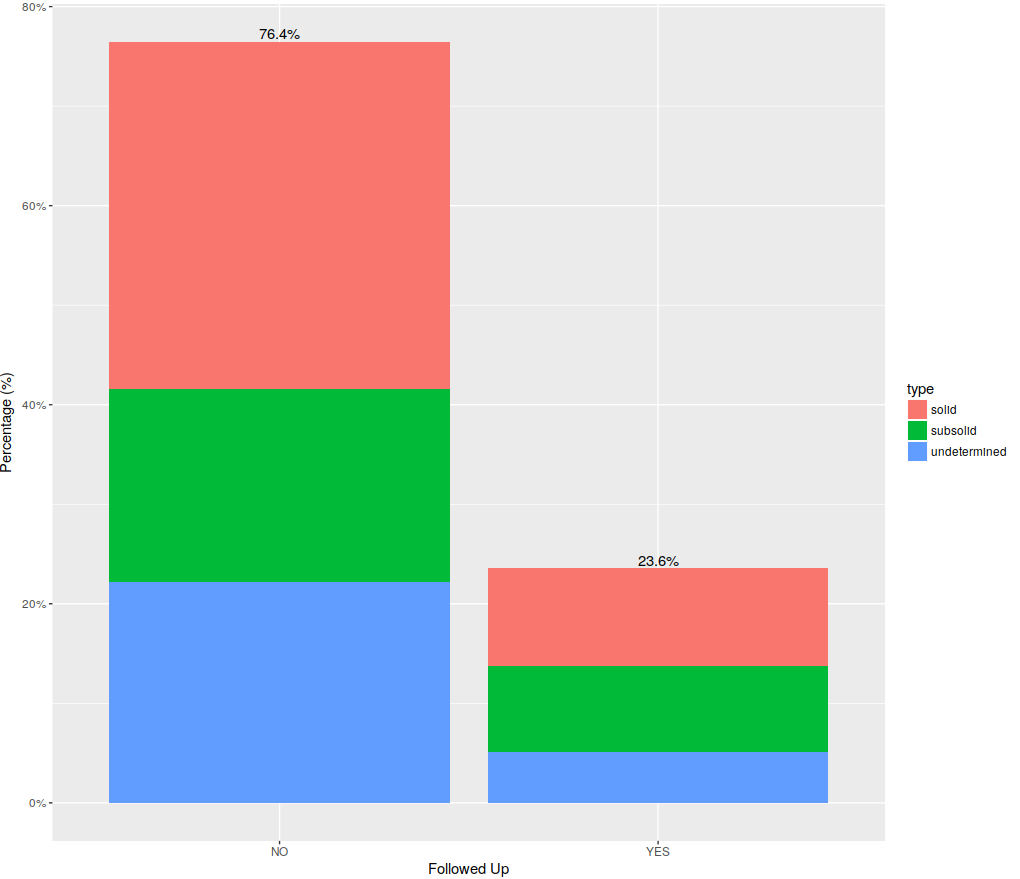
\includegraphics[height=0.26\textheight]{Reports_LungNoduleTypeFollowUp}
\end{centering}
\caption{\label{fig:reports_nodules}On the left, the number of nodules found in each of the different Fleischner table ranges (see tables~\ref{tab:solid_nodules} and~\ref{tab:subsolid_nodules}). On the right, a \emph{yes or no} flag view of the reports if they were a follow up to a previous report or not. On both cases the color information is the nodule type.}
\end{figure}
\vspace*{-44pt}
\end{center}

From the total lung nodule reports 22,900 (77.4\%) From these reports had nodules with less than 0.6 cm, 1,361 (4\%) were between 0.6 cm and 0.8 cm and 5325 (18\%) had more than 0.8 cm. Also, from the reports 22604 (76.4\%) were not follow up exams and 6982 (23.6\%) were. This can be seen in the figure~\ref{fig:reports_nodules}. On this figure the left side corresponds to the size ranges as observed in the Fleischner tables and the right side is the follow up exams. 

There is a concept of an \emph{undetermined} nodule type, which means that the NLP algorithm was unable to find any reporting information that described the nodule as either solid or subsolid. In this case, at least for \nomeHslShort{} data the default expected behavior in this case is that the data inference is of type \emph{solid} for these \emph{undetermined} nodules. This is so, because the sub-solidity of a nodule can only be atested if it is reported in the radiology report. That means that the absence of any term indicating a ground glass characteristic to the nodule means that it is solid.

\begin{center}
\begin{figure}
\begin{centering}
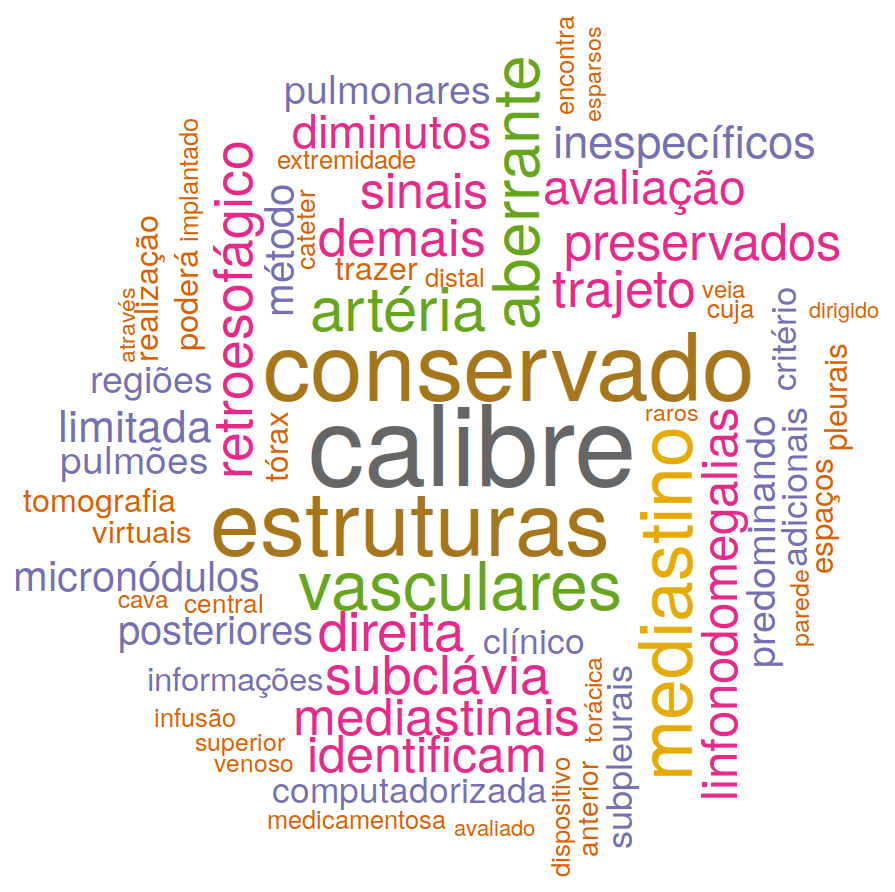
\includegraphics[width=0.495\textwidth]{Reports_AllReportsWordcloud}
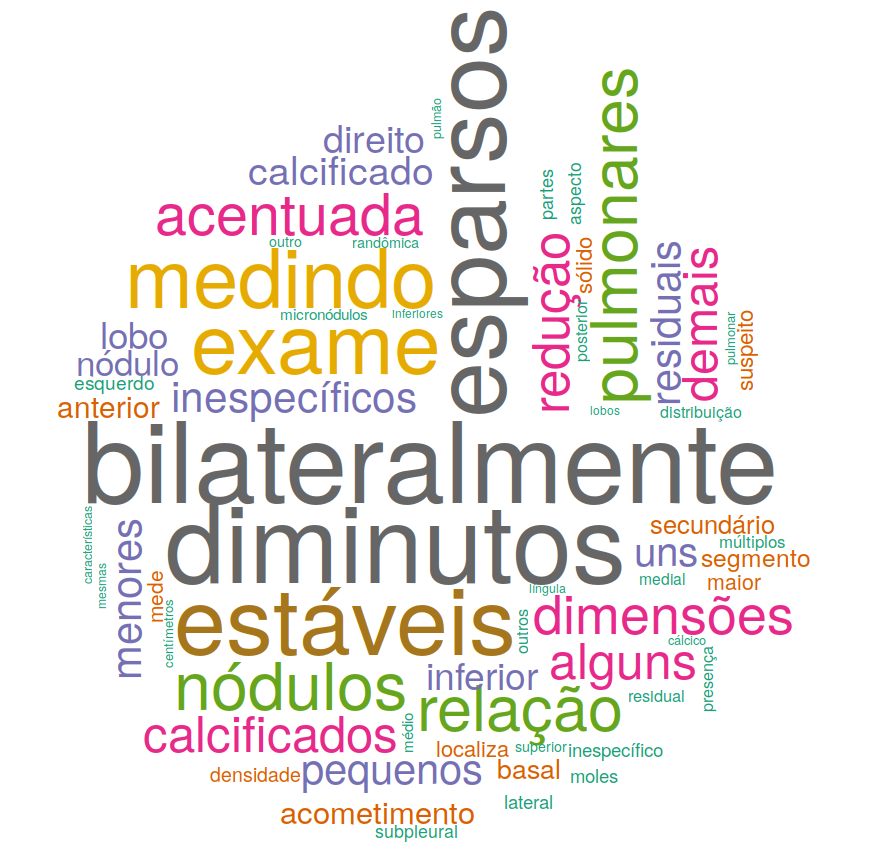
\includegraphics[width=0.495\textwidth]{Reports_OnlyLungNoduleReportsWordcloud}
\end{centering}
\caption{\label{fig:wordclouds}The left wordcloud represents all reports and their most frequent words, while the right one represents only the most frequent words in the sentences annotated by the NLP algorithm as a lung nodule.}
\end{figure}
\vspace*{-44pt}
\end{center}

Even more of interest, it is noticeable in the Fleischner tables that the nodules whose size are greater than 0.6 cm need an imaging follow-up regardless if they are of solid or subsolid types. This proves as an interesting mechanism to infer the number of patients and reports that actually should be followed up. 

If only the reports whose nodules are larger than 0.6 cm are taken into consideration the overall number of reports will be 8,754. From these, only 2,062 had an appropriate follow up according to the EHR information. This means that there are potentially 6,692 reports that did not have an appropriate follow up. These reports constitute a total of 2,201 patients that could be missing their indicated follow up according to the guideline.

From these reports, 3052 are of solid type, 1696 subsolid and 1944 undetermined, which as previously stated are the same as solid. That means 4996 solid nodules and 1696 subsolid are missing an adequate follow up into the \nomeHslShort{} EHR.

This analysis shows the potential impact that an incidental lung nodule screening program could have at \nomeHsl{}. Also, if the tabagism information from figure~\ref{fig:cigars_per_day} are taken into account. Only from that more than eight thousand patients could potentially be screened if both NCCN (table~\ref{tab:nccn_risk_lung_nodule} and Fleischner (tables~\ref{tab:solid_nodules} and~\ref{tab:subsolid_nodules}) guidelines are taken into consideration.

Finally, even with just the wordclouds from all CCT reports and only the sentences annotated as lung nodules, respectively left and right images from figure~\ref{fig:wordclouds}, one can see that terms easily related with pulmonary nodules such as lung locations and measurement indications are seen on the later more than on the first. Also on the first several vascular related words can be seen but not on the later. This is an interesting confirmation that the NLP algorithm is doing, at least in the general picture, a good job of filtering unrelated sentences and thus reports.
